\documentclass[a4paper,12pt]{article}

\usepackage[margin=2cm]{geometry}
\usepackage{graphicx}
\usepackage{amsmath}
\usepackage{array}
\usepackage{hyperref}
\usepackage[all]{hypcap}
\usepackage{listings}
\lstdefinestyle{TerminalStyle}{
  language=bash,
  basicstyle=\small\sffamily,
  numbers=left,
  numberstyle=\tiny,
  numbersep=3pt,
  frame=tb,
  columns=fullflexible,
  linewidth=0.9\linewidth,
  xleftmargin=0.1\linewidth
}
\lstdefinestyle{HtmlStyle}{
  language=html,
  basicstyle=\small\sffamily,
  numbers=left,
  numberstyle=\tiny,
  numbersep=3pt,
  frame=tb,
  columns=fullflexible,
  linewidth=0.9\linewidth,
  xleftmargin=0.1\linewidth
}
\lstdefinestyle{OutputStyle}{
  language=html,
  basicstyle=\small\sffamily,
  frame=tb,
  columns=fullflexible,
  linewidth=0.9\linewidth,
  xleftmargin=0.1\linewidth
}

\setlength{\parindent}{0pt}
\setlength{\parskip}{1ex plus 0.5ex minus 0.2ex}

\title{
\includegraphics[width=12cm]{Eeufeeslogo.jpg} \\
       Department of Computer Science \\
       University of Pretoria \\
       \vspace{0.5cm}
       COS730 Software Engineering \\
       \vspace{0.5cm}
       \begin{large} \textbf{Software Requirement Specifications}\end{large}}

\date{} 
\author{	JM Bondjobo		13232852 		\\
		Martha Mohlala		10353403
		D Jansen van Vuuren	18364412
		 \\
		 KJ Muranga         13278012        \\
		 RT Mabaso          18296272
}

\begin{document}
\maketitle
\thispagestyle{empty}
\clearpage

\newpage
\pagenumbering{roman}
\thispagestyle{empty}
\tableofcontents
\clearpage

\newpage
\pagenumbering{arabic}

\section {Introduction}
This section gives a scope description of the benchmark service system. Also, the purpose for this document is described and a list of abbreviations and definitions is provided.
\subsection{Purpose}
The goal of this document is to give a detailed description of the  benchmarking service. It will explain the purpose and features of the system, the interfaces of the system, what the system will do and the constraints under which it must operate.


\subsection{Scope}
The benchmarking service will accept a user's source code and measure its performance in terms of CPU time, elapsed time, memory usage, power consumption, heat generation, and others.The user's source code could be either an algorithm or a data structure, and the system should give the user a choice of which programming languages their source code can be implemented in. The service should be provided by executing the requested benchmarks on isolated machines where the side-effects that are not a concern of the specified benchmark are minimized.

The system will be used as an integral part of research related to the development of new algorithms and techniques as well as the refinement and optimisation of existing operations. It can also be used to as a teaching tool for students to review the notions of space and time complexity.



\subsection{Definitions, Acronyms and Abbreviations}
\begin{center}
\begin{tabular}{ |p{5cm}|p{10cm}| } 
\hline
Term & Definition \\ 
\hline
User & Individual who uses the benchmarking system. \\ 
\hline
Software Requirements Specification & A document that completely describes all of the functions of a proposed system and the constraints under which it must operate. For example, this document. \\ 
\hline
Benchmark & Evaluate (something) by comparison with a standard. \\
\hline
RAM & Random Access Memory  \\
\hline
HTTP & HyperText Transfer Protocol \\
\hline
\end{tabular}
\end{center}

\subsection{References}
IEEE. IEEE Std 830-1998 IEEE Recommended Practice for Software Requirements Specifications. IEEE Computer Society, 1998

\subsection{Overview}
The remainder of this document consists of two chapters. The second chapter, the Overall Description section, of this document gives a description of the system's functionality. It describes the informal requirements and is used to establish a context for the technical requirements specification in the next chapter.

The third chapter, Specific Requirements section, of this document gives a detailed description of the benchmarking service. It describes in technical terms the details of the functionality of the system.

\section{Overall Description}



\subsection{Product Perspective}

\subsubsection{System Interfaces}
The system will provide a web interface for users to request and specify the benchmarking services they need. The system interface is depicted as below:\\
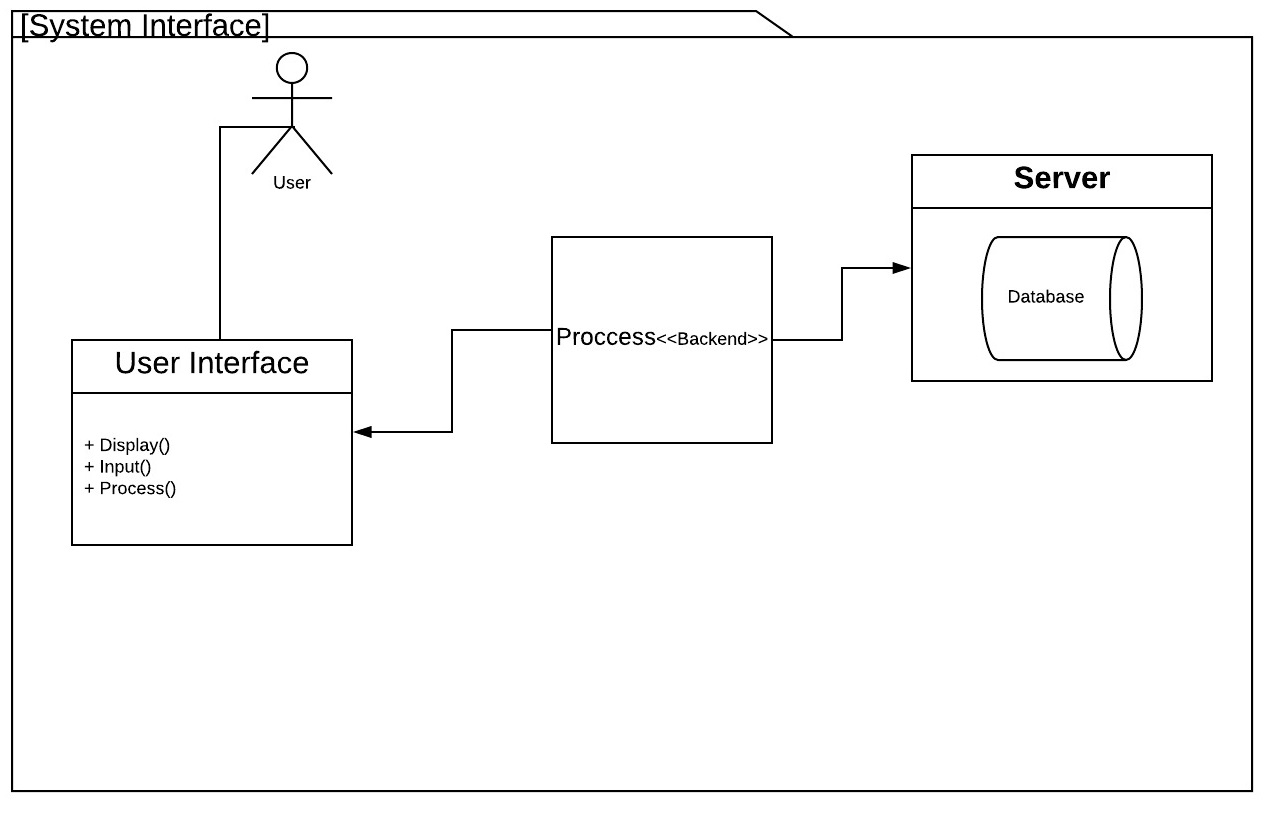
\includegraphics[width=12cm]{SI.jpeg}
\subsubsection{User Interfaces}
The system will have a user interface where s/he is interacting with the system by requesting some services and getting a response from the system done at the backend. This is the front end part of the system that the client/user will be seing. It must follow basic Windows style and functionality conventions. The interface will have a menu where the services can be requested, a log button on the menu to see what services were done on the pc and by who and a quick access button to terminate the benchmarking process if something goes wrong.
\subsubsection{Hardware Interfaces}
The system will run a computer that has is Windows 7 and higher and that has at least 100 Mb of free space on the hard drive and 1Gb of Ram. That pc used must be an isolated machine where the benchmarking service will be done in order to reduce/ minimize the side effects of others programs running simultaneously. The system does not write information directly to the user's computer. But instead uses a database which is located on a network server. The user's computer transfers and receives data using basic networking protocols like HTTP. All systems' information is stored in the server's database which stores the data on the server's disk reason being if the system runs out of memory or fails during benchmarking the previously gathered information remains on the server's database.
\subsubsection{Softwares Interfaces}
The system requires a a properly configuered version of Windows 7 or later to run the application. The system's server can either be Windows or Linux but must have a MySQL databse properly installed and configured. The software interface will be web based, therefore must have Microsoft .NET Framework 1.1 or greater installed and for the designing of the benchmarking that can be done using Adobe XD.

\subsubsection{Communications Interfaces}
The benchmarking system will have a network server that is web-based. The server exists to retrieve information from the database
and compute the services in terms of the benchmark metrics provided. The web interface will also query the database for the historical computations of the benchmark metrics. The HTTP server will be used to send the requests from the web interface to
the benchmarking system. The web application will support all types of browsers.
\subsubsection{Memory}
The system will not use memory less than 100Mb of the hard drive and 1Gb of RAM as described on the hardware interface.
\subsubsection{Operations}
The user will initiate the request for benchmarking services and wait for response. The response might take a while as the system is required to do computation and comparison between two inputs. The user will have an option of inputting algorithm or data structure and the input will be validated to check if it is algorithm or data structure. The system will also allow the user to store all the computation and comparison results to the database as historical data to avoid computing the same request many times,and also for recovery. 
\subsubsection{Site Adaptation Requirements}
The program/tool must able to view and compile code. It must measure CPU (Central Processing Unit) performance, memory usage (RAM, Random Access Memory), temperature, power consumption and a lot of other variables.
It should also ideally be able to accept and handle any modern coding languages such as Java, C#, C++ etc. The program must also be a web-application that can compile code and test for its runtime attributes. 
The user must select their programming language and then input the code. The program then compiles the code and give feedback on power usage, temperature difference etc. This will all be done in a web-application.

\subsection{Product Functions}
The software will perform a list of functions like:
-	Check what code is written.
-	Compile code
-	Minimize main application concern
-	Calculate memory usage
-	Calculate temperature difference
-	Calculate power consumption
-	Calculate CPU usage
-	Give feedback.
-	User must be able to keep feedback (download)
These functions must be executed and the correct feedback must be given. For instance, when the user’s code is compiled, the calculation must not measure performance changes to the program, but rather only to the user’s code. 
The process of the functions are as follows:
1.	User select’s programming language
2.	User inputs their code.
3.	Program compiles code.
4.	Measure performance and hold information
5.	If code did not have any errors
a.	Give performance feedback
6.	If code did have errors
a.	Give correct feedback

\subsection{User Characteristics}
An average user does not even need to have a programming background. If the user needs to test the performance of code and give the feedback back to the developer, they can. They can simply copy the code into the program and get the results, if there aren’t any errors in the code that they submitted. One of the goals of the application is to give feedback in a very user friendly manner, so that they do not need any knowing of how coding works to use the information. 

Graphs can be created to give users an even better understanding of how the application measures performance. These graphs can then be downloaded and exported to an excel document or PDF. 

\subsection{Constraints}
Limitations to developer options can include the following:
-	Programming knowledge (Being able to only compile code that the developers know of.)
-	Parallel operation (Measuring one program inside another program.)
-	Control function (Test whether user code will “break” our program.)
-	If user’s device is to slow (Hinder measuring process may result in inaccurate results.)

\subsection{Assumptions and Dependencies}

\section{Specific Requirements}

\subsection{External Interface Requirements}

\subsection{Functional Requirements}

\subsection{Performance Requirements}
The system shall respond to user input in few minutes, if it takes too long than expected, a progress indicator shall be display to notify the user.
If the system loses the connection to internet, an error message or pop-up message will be display to inform the user.
The system should be able to handle reasonable users without inconsistency.
\subsection{Design Constraints}
The hard drive free space must be at least 100MB and 1GB ram.
\subsection{Software System Attributes}
\subsubsection{Reliability}
The system should work reliably, with automatic backup and recovery features. In case of unexpected operating system error or shut-down, the unsaved data should be recovered without loss. The user will be able to save all the computation and comparison results to the database.
\subsubsection{Availability}
The system will be available when it is used.The internet connection should be available to use the system.
\subsubsection{ Security }
The system should be access only by the authenticated users. The users credential should be encrypted.\subsubsection{Maintainability}
All code shall be well documented. Each function will have comment so that it can be easy for the developer who wishes to edit it and for the person who is in charge for maintenance.
\subsubsection{Portability}
The system should support windows 7 and higher.
\subsubsection{Usability}
 The GUI should be easy to learn and use by users. Either user has programming background or not the system should be user friendly. A built-in help feature should be available in all pages, to guide users how the system work and how to use the system.
\subsection{Other Requirements}

\newpage
\clearpage
\addcontentsline{toc}{section}{References}

\end{document}
